\section{Reagenti}
Indica il tipo e le caratteristiche dei reagenti  impiegati (è essenziale segnalare la concentrazione delle soluzioni e, per i solidi, il grado di purezza).
Nel caso i reagenti disponessero di una scheda di sicurezza è buona norma riportare in maniera sintetica tali informazioni come pittogrammi, frasi H e P, i DPI necessari la TLV.

A questo scopo viene mostrato anche come mettere le equazioni e formule chimiche con un pacchetto apposito:
\begin{itemize}
    \item \ce{H3PO4} 0.3 M 25 mL
\end{itemize}

\begin{table}[!ht]
    \scriptsize
    \centering
    \begin{tabularx}{\textwidth}{m{0.15\textwidth}|m{0.2\textwidth}|m{0.23\textwidth}|m{0.17\textwidth}|m{0.13\textwidth}}
        \toprule
        \textbf{Composto}                                                                                                                                                                                                                 & \textbf{Formula di struttura}                                                 & \textbf{Frasi H e P}       & \textbf{Pittogrammi} & \textbf{DPI} \\
        \midrule
        \ce{H2O2}                                                                                                                                                                                                                         & \begin{center}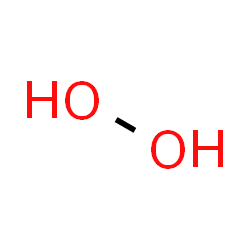
\includegraphics[width=3cm,scale=0.4]{img/763.png} \end{center} &
        H: H271, H302, H314 e H332.

        P: P210, P220, P221, P260, P261, P264, P270, P271, P280, P283, P301+P312, P301+P330+P331, P303+P361+P353, P304+P312, P304+P340, P305+P351+P338, P306+P360, P310, P312, P321, P330, P363, P370+P378, P371+P380+P375, P405, e P501. & \begin{center} \begin{tabular}{cc}
                
\includegraphics[scale=0.15]{img/pittogrammi/Flammable.png} & 
\includegraphics[scale=0.15]{img/pittogrammi/Explosive.png} \\
                
\includegraphics[scale=0.15]{img/pittogrammi/Flammable.png} & 
\includegraphics[scale=0.15]{img/pittogrammi/Explosive.png}
            \end{tabular}\end{center}                          & guanti, occhiali e visiera                                       \\
        \bottomrule
    \end{tabularx}
    \caption{Tabella con i composti chimici utilizzati nell'esperienza, le frasi P e H vengono riportate per esteso al fondo della relazione.} % da modificare
    \label{tab:tab1} % da modificare
    \normalsize
\end{table}

\newpage
Tabella precedente con i TLV (threshold limit value) che sono valori di concentrazione di sostanze aerodisperse, più o meno tossiche, al di sotto delle quali la maggior parte dei lavoratori può rimanere esposta ripetutamente tutti giorni senza effetti dannosi per la salute.

\begin{table}[!ht]
    \centering
    \scriptsize
    \begin{tabularx}{1\textwidth}{m{0.15\textwidth}|m{0.15\textwidth}|m{0.2\textwidth}|m{0.12\textwidth}|m{0.1\textwidth}|m{0.13\textwidth}}
        \toprule
        \textbf{Composto}                                                                                                             & \textbf{Formula di struttura}                                                            & \textbf{Frasi H e P}                         & \textbf{Pittogrammi} & \textbf{DPI} & \textbf{TLV [ppm]} \\
        \midrule
        \ce{H2O2}                                                                                                                     & \begin{center}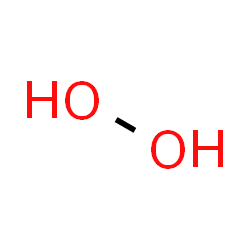
\includegraphics[width=0.15\textwidth,scale=0.4]{img/763.png} \end{center} & \Hphrase{H271} \Hphrase{H302} \Pphrase{P261} &
        \begin{tabular}{c}
            
\includegraphics[scale=0.15]{img/pittogrammi/Flammable.png} \\ 
\includegraphics[scale=0.15]{img/pittogrammi/Explosive.png} \\
            
\includegraphics[scale=0.15]{img/pittogrammi/Flammable.png} \\ 
\includegraphics[scale=0.15]{img/pittogrammi/Explosive.png}
        \end{tabular} & guanti, occhiali e visiera                                                               & LTEL: 100

        STEL: 200                                                                                                                                                                                                                                                                                                                          \\
        \bottomrule
    \end{tabularx}
    \caption{Tabella con i composti chimici utilizzati nell'esperienza, le frasi P e H vengono riportate per esteso al fondo della relazione. Ricorda che: Long-term Exposure Limit (LTEL) Values e Short-term Exposure Limit (STEL) Values} % da modificare
    \label{tab:tab2} % da modificare
    \normalsize
\end{table}

Oppure, in alcuni casi, è necessaria una tabella differente come la seguente.

Esprime i rapporti stechiometrici, le masse e le rese, utili nelle reazioni di sintesi quando si deve capire il meccanismo e quest'ultimo può variare in base alle concentrazioni dei reagenti.

\begin{table}[ht]
    \centering
    \scriptsize
    \begin{tabularx}{1\textwidth}{X|X|X|X|X|X|X|X|X}
        \toprule
        Sostanza & Massa molecolare\newline[g/mol] & Moli\newline[mol] & Rapporto stechiometrico & Massa\newline[g] & Volume\newline[mL] & Resa\newline[\%] & Frasi H & Frasi P \\
        \midrule
        A        & B                               & C                 & D                       & E                & F                  & G                & H       & I       \\
        \bottomrule
    \end{tabularx}
    \caption{Tabella per sintesi}
    \label{tab:tab3}
    \normalsize
\end{table}

\begin{table}[ht]
    \centering
    \scriptsize
    \begin{tabularx}{1\textwidth}{X|X|X|X|X|X|X}
        \toprule
        Composto & Struttura & Aspetto          & Rischi  & Protezioni & TLV/TWA     & Smaltimento                         \\
        \midrule
        \ce{H2O} &           & liquido incolore & nessuno & nessuna    & irrilevante & semplicemente gettare nel lavandino \\
        \midrule
        \ce{H2O} &           & liquido incolore & nessuno & nessuna    & irrilevante & semplicemente gettare nel lavandino \\
        \midrule
        \ce{H2O} &           & liquido incolore & nessuno & nessuna    & irrilevante & semplicemente gettare nel lavandino \\
        \midrule
        \ce{H2O} &           & liquido incolore & nessuno & nessuna    & irrilevante & semplicemente gettare nel lavandino \\
        \bottomrule
    \end{tabularx}
    \caption{Altro modello di tabella.}
    \label{tab:my_label}
\end{table}

Per i DPI si è costretti a cercare il nome del composto e scrivere di seguito scheda di sicurezza su un qualsiasi motore di ricerca e cercando il risultato più recente.

\info[inline]{es. acido benzoico scheda di sicurezza.}

Ricordarsi il produttore, facendo una foto in laboratorio del contenitore, può accelerare il lavoro ed essere più corretti in quanto le informazioni potrebbero non sempre essere uguali.
In fondo alla scheda si trova, oltre alle informazioni sui DPI, altre varie informazioni utili.
